\documentclass[12pt]{article}
\usepackage[utf8]{inputenc}
\usepackage[catalan]{babel}
\usepackage{amsmath, amssymb, amsfonts}
\usepackage{geometry}
\usepackage{fancyhdr}
\usepackage{graphicx}
\usepackage{tikz}
\usetikzlibrary{matrix, calc}
\usepackage{tcolorbox}
\usepackage[colorlinks=true, linkcolor=blue]{hyperref}
\usepackage{float}
\usepackage{enumitem}

\setlength{\headheight}{15pt}

\geometry{a4paper, left=2cm, right=2cm, top=2.5cm, bottom=2.5cm}

\pagestyle{fancy}
\fancyhf{}
\fancyhead[L]{Matemàtiques 2n Batxillerat}
\fancyhead[R]{Càlcul integral: Integrals}
\fancyfoot[L]{\href{mailto:orodri11@xtec.cat}{orodri11@xtec.cat}}
\fancyfoot[R]{\thepage}

% Colors més suaus per a llegibilitat en impressió
\newtcolorbox{concept}[1][]{colback=blue!5!white, colframe=blue!75!black, fonttitle=\bfseries, title=Concepte, #1}
\newtcolorbox{exemple}[1][]{colback=green!5!white, colframe=green!75!black, fonttitle=\bfseries, title=Exemple, #1}
\newtcolorbox{exercici}[1][]{colback=yellow!10!white, colframe=yellow!75!black, fonttitle=\bfseries, title=Exercici, #1}
\newtcolorbox{solucio}[1][]{colback=orange!5!white, colframe=orange!75!black, fonttitle=\bfseries, title=Solució, #1}

\begin{document}

\begin{titlepage}
    \centering
    \vspace*{1cm}
    {\Huge \textbf{Càlcul Integral: \\ Les Integrals i les seves aplicacions} \par}
    \vspace{0.5cm}
    {\Large Matemàtiques 2n Batxillerat \par}
    \vspace{1.5cm}
    % Substituir per la imatge real
    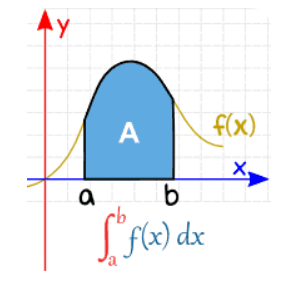
\includegraphics[width=0.5\textwidth]{integrals.png} 
    \vspace{1.5cm}
    \tableofcontents
\end{titlepage}

\newpage

\section{Integrals indefinides}

\subsection{Primitiva d'una funció}

\begin{concept}
\textbf{Definició de primitiva}\\
Direm que $F(x)$ és una \textbf{primitiva} de $f(x)$ si:
\[
\boxed{F'(x) = f(x)}
\]

És a dir, una primitiva de $f$ és una funció que, derivada, dóna $f$.
\end{concept}

\begin{exemple}
\textbf{Exemple 1: Primitives de $f(x)=x^2$}\\
Cal buscar una funció $F(x)$ tal que derivant-la doni $x^2$. Veiem que haurà de ser un polinomi de grau 3:
\[
F(x)=\frac{x^3}{3}
\]
és una primitiva de $f(x)$, però
\[
F(x)=\frac{x^3}{3}+5
\]
també ho és. Ambdues funcions, en derivar-les, donen $f(x)=x^2$.

Per tant, podem afirmar que:
\[
\boxed{\text{Totes les primitives d'una funció difereixen només en una constant.}}
\]
\end{exemple}

\subsection{Definició: Integral indefinida}

\begin{concept}
\textbf{Integral indefinida}\\
Es defineix la \textbf{integral indefinida} d'una funció com el conjunt de totes les primitives d'aquesta funció i es representa de la manera següent:
\[
\boxed{\int f(x)\,dx = F(x) + C}
\]
on $C$ és una constant (anomenada \textbf{constant d'integració}).
\end{concept}

\subsection{Taula d'integrals indefinides immediates}

\begin{concept}
\textbf{Integrals immediates bàsiques}

\vspace{0.3cm}

\renewcommand{\arraystretch}{1.4}
\begin{center}
\begin{tabular}{|l|l|}
\hline
\textbf{Funció} & \textbf{Integral} \\
\hline
$k$ (constant) & $\displaystyle \int k\,dx = kx + C$ \\
$x^n$ & $\displaystyle \int x^n\,dx = \dfrac{x^{n+1}}{n+1} + C$ \quad $(n\neq -1)$ \\
$\dfrac{1}{x}$ & $\displaystyle \int \dfrac{1}{x}\,dx = \ln|x| + C$ \\
$e^x$ & $\displaystyle \int e^x\,dx = e^x + C$ \\
$a^x$ & $\displaystyle \int a^x\,dx = \dfrac{a^x}{\ln a} + C$ \\
$\sin x$ & $\displaystyle \int \sin x\,dx = -\cos x + C$ \\
$\cos x$ & $\displaystyle \int \cos x\,dx = \sin x + C$ \\
$\sec^2 x$ & $\displaystyle \int \sec^2 x\,dx = \tan x + C$ \\
$\dfrac{1}{1+x^2}$ & $\displaystyle \int \dfrac{1}{1+x^2}\,dx = \arctan x + C$ \\
$\dfrac{1}{\sqrt{1-x^2}}$ & $\displaystyle \int \dfrac{1}{\sqrt{1-x^2}}\,dx = \arcsin x + C$ \\
\hline
\end{tabular}
\end{center}
\end{concept}

\begin{exemple}
\textbf{Exemple 2: Compte amb les constants!}\\
Calculem $\displaystyle \int \dfrac{1}{2x}\,dx$.

Tal com hem vist, totes les primitives d'una funció difereixen en una constant. Però aquí sembla que no es compleixi aquesta regla. Podem integrar aquesta funció de dues maneres diferents:
\[
\int \dfrac{1}{2x}\,dx =
\begin{cases}
\dfrac{1}{2}\displaystyle\int \dfrac{2}{2x}\,dx = \dfrac{1}{2}\ln(2x) + C_1 \\[0.3cm]
\dfrac{1}{2}\displaystyle\int \dfrac{1}{x}\,dx = \dfrac{1}{2}\ln x + C_2
\end{cases}
\]
Semblaria que les dues funcions són diferents i que hi hauria dues primitives per a la mateixa funció. Però veiem que són la mateixa i només difereixen en una constant. Aplicant les lleis dels logaritmes a la primera expressió:
\[
\dfrac{1}{2}\ln(2x)+C_1 = \dfrac{1}{2}(\ln 2 + \ln x)+C_1 = \dfrac{\ln 2}{2}+\dfrac{1}{2}\ln x+C_1 = \dfrac{1}{2}\ln x+C'
\]
ja que $\ln 2$ és un nombre real. Per tant, acabem de veure que les dues primitives són la mateixa i només difereixen en una constant.
\end{exemple}

\subsection{Taula d'integrals indefinides quasi-immediates}

\begin{concept}
\textbf{Integrals quasi-immediates}\\
Considerem $u(x)$ una funció qualsevol. Llavors:

\renewcommand{\arraystretch}{1.5}
\begin{center}
\begin{tabular}{|l|l|}
\hline
\textbf{Integral} & \textbf{Resultat} \\
\hline
$\displaystyle \int \dfrac{u'(x)}{u(x)}\,dx$ & $\ln|u(x)| + C$ \\
$\displaystyle \int e^{u(x)} \cdot u'(x)\,dx$ & $e^{u(x)} + C$ \\
$\displaystyle \int u(x)^n \cdot u'(x)\,dx$ & $\dfrac{u(x)^{n+1}}{n+1} + C$ \quad $(n\neq -1)$ \\
$\displaystyle \int \cos(u(x)) \cdot u'(x)\,dx$ & $\sin(u(x)) + C$ \\
$\displaystyle \int \sin(u(x)) \cdot u'(x)\,dx$ & $-\cos(u(x)) + C$ \\
$\displaystyle \int \sec^2(u(x)) \cdot u'(x)\,dx$ & $\tan(u(x)) + C$ \\
$\displaystyle \int \dfrac{u'(x)}{1+u(x)^2}\,dx$ & $\arctan(u(x)) + C$ \\
$\displaystyle \int \dfrac{u'(x)}{\sqrt{1-u(x)^2}}\,dx$ & $\arcsin(u(x)) + C$ \\
\hline
\end{tabular}
\end{center}
\end{concept}

\subsection{Propietats de les integrals indefinides}

\begin{concept}
\textbf{Propietats de linealitat}\\
Les integrals indefinides compleixen les següents propietats:

\begin{enumerate}
    \item \textbf{Suma:} $\displaystyle \int (f(x) + g(x))\,dx = \int f(x)\,dx + \int g(x)\,dx$
    \item \textbf{Producte per una constant:} $\displaystyle \int k \cdot f(x)\,dx = k \cdot \int f(x)\,dx, \quad k \in \mathbb{R}$
\end{enumerate}
\end{concept}

\subsection{Més exemples d'integrals indefinides quasi-immediates}

\begin{exemple}
\textbf{Exemple 3: $\displaystyle \int \cot x\,dx$}\\
\[
\int \cot x\,dx = \int \dfrac{\cos x}{\sin x}\,dx = \ln|\sin x| + C
\]
\end{exemple}

\begin{exemple}
\textbf{Exemple 4: $\displaystyle \int \tan x\,dx$}\\
\[
\int \tan x\,dx = \int \dfrac{\sin x}{\cos x}\,dx = -\ln|\cos x| + C
\]
\end{exemple}

\begin{exemple}
\textbf{Exemple 5: $\displaystyle \int \dfrac{x}{3x^2+5}\,dx$}\\
\[
\int \dfrac{x}{3x^2+5}\,dx = \dfrac{1}{6} \ln(3x^2+5) + C
\]
\end{exemple}

\begin{exemple}
\textbf{Exemple 6: $\displaystyle \int x \sqrt[3]{3x^2+1}\,dx$}\\
\[
\int x (3x^2+1)^{1/3}\,dx = \dfrac{(3x^2+1)^{4/3}}{8} + C
\]
\end{exemple}

\begin{exemple}
\textbf{Exemple 7: $\displaystyle \int \dfrac{\ln x}{x}\,dx$}\\
\[
\int \dfrac{\ln x}{x}\,dx = \dfrac{\ln^2 x}{2} + C
\]
\end{exemple}

% ---------------------------------------------------------
% MÈTODES D'INTEGRACIÓ
% ---------------------------------------------------------
\section{Mètodes d'integració}

\subsection{Integració de funcions racionals}

\begin{exemple}
\textbf{Exemple 8: $\displaystyle \int \frac{dx}{(x-a)^n}$}\\
\[
\int \frac{dx}{(x-a)^n} = \frac{1}{(1-n)(x-a)^{n-1}} + C
\]
\end{exemple}

\begin{exemple}
\textbf{Exemple 9: $\displaystyle \int \frac{1}{b+cx^2}\,dx$}\\
\[
\int \frac{1}{b+cx^2}\,dx = \frac{1}{\sqrt{bc}} \arctan\left(\sqrt{\frac{c}{b}}x\right) + C
\]
\end{exemple}

\begin{exemple}
\textbf{Exemple 10: $\displaystyle \int \frac{x+2}{x-3}\,dx$}\\
\[
\int \frac{x+2}{x-3}\,dx = x + 5\ln|x-3| + C
\]
\end{exemple}

\begin{exemple}
\textbf{Exemple 11: $\displaystyle \int \frac{x^2-2x}{x^3-3x^2+1}\,dx$}\\
\[
\int \frac{x^2-2x}{x^3-3x^2+1}\,dx = \frac{1}{3} \ln|x^3-3x^2+1| + C
\]
\end{exemple}

\begin{exemple}
\textbf{Exemple 12: $\displaystyle \int \frac{x^3-4}{x^2-x-2}\,dx$}\\
Primer fem la divisió:
\[
\frac{x^3-4}{x^2-x-2} = x+1 + \frac{3x-2}{x^2-x-2}
\]
Ara descomponem la fracció:
\[
\frac{3x-2}{(x+1)(x-2)} = \frac{A}{x-2} + \frac{B}{x+1}
\]
Resolem:
\[
3x-2 = A(x+1) + B(x-2)
\]
Per $x=2$: $A=\frac{4}{3}$. Per $x=-1$: $B=\frac{5}{3}$.

Per tant:
\[
\int \frac{x^3-4}{x^2-x-2}\,dx = \frac{x^2}{2} + x + \frac{4}{3}\ln|x-2| + \frac{5}{3}\ln|x+1| + C
\]
\end{exemple}

\begin{exemple}
\textbf{Exemple 13: $\displaystyle \int \frac{1}{4x^2-4x+5}\,dx$}\\
Completant quadrats:
\[
4x^2-4x+5 = 4\left(x-\frac{1}{2}\right)^2 + 4
\]
Per tant:
\[
\int \frac{1}{4x^2-4x+5}\,dx = \frac{1}{4}\arctan\left(x-\frac{1}{2}\right) + C
\]
\end{exemple}

\subsection{Integració per parts}

\begin{concept}
\[
\int f(x)g'(x)\,dx = f(x)g(x) - \int f'(x)g(x)\,dx
\]
\end{concept}

\begin{exemple}
\textbf{Exemple 14: $\displaystyle \int x\sin(2x)\,dx$}\\
Fem $u=x$, $dv=\sin(2x)dx$. Llavors $du=dx$, $v=-\frac{1}{2}\cos(2x)$. Aplicant la fórmula:
\[
\int x\sin(2x)\,dx = x\left(-\frac{1}{2}\cos(2x)\right) - \int \left(-\frac{1}{2}\cos(2x)\right) dx = -\frac{x}{2}\cos(2x) + \frac{1}{2}\int \cos(2x)\,dx
\]
\[
= -\frac{x}{2}\cos(2x) + \frac{1}{2}\cdot\frac{1}{2}\sin(2x) + C = -\frac{x}{2}\cos(2x) + \frac{1}{4}\sin(2x) + C
\]
\end{exemple}

\begin{exemple}
\textbf{Exemple 15: $\displaystyle \int x^2\sin(3x)\,dx$}\\
Aplicant integració per parts dues vegades:

Primera: $u=x^2$, $dv=\sin(3x)dx$ $\Rightarrow du=2x\,dx$, $v=-\frac{1}{3}\cos(3x)$.
\[
\int x^2\sin(3x)\,dx = -\frac{x^2}{3}\cos(3x) + \frac{2}{3}\int x\cos(3x)\,dx
\]

Segona: per a $\int x\cos(3x)\,dx$, fem $u=x$, $dv=\cos(3x)dx$ $\Rightarrow du=dx$, $v=\frac{1}{3}\sin(3x)$.
\[
\int x\cos(3x)\,dx = \frac{x}{3}\sin(3x) - \int \frac{1}{3}\sin(3x)\,dx = \frac{x}{3}\sin(3x) + \frac{1}{9}\cos(3x)
\]

Substituint:
\[
\int x^2\sin(3x)\,dx = -\frac{x^2}{3}\cos(3x) + \frac{2}{3}\left( \frac{x}{3}\sin(3x) + \frac{1}{9}\cos(3x) \right) + C
\]
\[
= -\frac{x^2}{3}\cos(3x) + \frac{2x}{9}\sin(3x) + \frac{2}{27}\cos(3x) + C
\]
\end{exemple}

\subsection{Mètode de substitució}

\begin{exemple}
\textbf{Exemple 16: $\displaystyle \int \frac{dx}{x\sqrt{x^2-1}}$}\\
Canvi $t = \sqrt{x^2-1}$. Llavors:
\[
dx = \frac{t}{x}\,dt, \qquad x^2 = t^2+1
\]
Substituint:
\[
\int \frac{dx}{x\sqrt{x^2-1}} = \int \frac{1}{x \cdot t} \cdot \frac{t}{x}\,dt = \int \frac{dt}{x^2} = \int \frac{dt}{t^2+1} = \arctan t + C = \arctan(\sqrt{x^2-1}) + C
\]
\end{exemple}

\begin{exemple}
\textbf{Exemple 17: $\displaystyle \int \sqrt{16-x^2}\,dx$}\\
Canvi $x = 4\sin t$, amb $t \in [-\pi/2, \pi/2]$. Llavors $dx = 4\cos t\,dt$ i $\sqrt{16-x^2} = \sqrt{16-16\sin^2 t} = 4\cos t$ (positiu). Substituint:
\[
\int \sqrt{16-x^2}\,dx = \int 4\cos t \cdot 4\cos t\,dt = 16\int \cos^2 t\,dt
\]
Usem $\cos^2 t = \frac{1+\cos 2t}{2}$:
\[
16\left( \frac{t}{2} + \frac{\sin 2t}{4} \right) + C = 8t + 4\sin 2t + C
\]
Desfent el canvi: $t = \arcsin(x/4)$, $\sin 2t = 2\sin t\cos t = 2\cdot \frac{x}{4} \cdot \frac{\sqrt{16-x^2}}{4} = \frac{x\sqrt{16-x^2}}{8}$. Per tant:
\[
= 8\arcsin\left(\frac{x}{4}\right) + 4\cdot \frac{x\sqrt{16-x^2}}{8} + C = 8\arcsin\left(\frac{x}{4}\right) + \frac{x}{2}\sqrt{16-x^2} + C
\]
\end{exemple}

\begin{exemple}
\textbf{Exemple 18: $\displaystyle \int \frac{1+e^x}{1-e^x}\,dx$}\\
Canvi $t = e^x$. Llavors $dx = \frac{dt}{t}$:
\[
\int \frac{1+e^x}{1-e^x}\,dx = \int \frac{1+t}{t(1-t)}\,dt
\]
Descomponent en fraccions parcials:
\[
\frac{1+t}{t(1-t)} = \frac{A}{t} + \frac{B}{1-t} \Rightarrow 1+t = A(1-t) + Bt
\]
Per $t=0$: $A=1$. Per $t=1$: $2 = B \Rightarrow B=2$. Per tant:
\[
= \int \left( \frac{1}{t} + \frac{2}{1-t} \right) dt = \ln|t| - 2\ln|1-t| + C = x - 2\ln(1-e^x) + C
\]
\end{exemple}


% ---------------------------------------------------------
% INTEGRALS TRIGONOMÈTRIQUES
% ---------------------------------------------------------
\section{Integrals trigonomètriques}

Anomenem \textbf{integrals trigonomètriques} aquelles on en l'integrand hi ha una combinació de funcions trigonomètriques.

\subsection{Integrals del tipus \(\displaystyle \int \sin^p x \cdot \cos^q x\,dx\) amb $p$ i $q$ parells}

Per a aquestes integrals, utilitzarem les fórmules trigonomètriques:
\[
\cos^2 x = \frac{1+\cos 2x}{2}, \qquad \sin^2 x = \frac{1-\cos 2x}{2}
\]

\begin{exemple}
\textbf{Exemple 19: $\displaystyle \int \sin^2 x\,dx$}\\
Usant la identitat:
\[
\int \sin^2 x\,dx = \int \frac{1-\cos 2x}{2}\,dx = \frac{x}{2} - \frac{\sin 2x}{4} + C
\]
\end{exemple}

\begin{exemple}
\textbf{Exemple 20: $\displaystyle \int \sin^4 x\,dx$}\\
\[
\sin^4 x = (\sin^2 x)^2 = \left(\frac{1-\cos 2x}{2}\right)^2 = \frac{1 - 2\cos 2x + \cos^2 2x}{4}
\]
Ara, $\cos^2 2x = \frac{1+\cos 4x}{2}$. Per tant:
\[
\sin^4 x = \frac{1}{4} - \frac{1}{2}\cos 2x + \frac{1}{8}(1+\cos 4x) = \frac{3}{8} - \frac{1}{2}\cos 2x + \frac{1}{8}\cos 4x
\]
Integrant:
\[
\int \sin^4 x\,dx = \frac{3x}{8} - \frac{\sin 2x}{4} + \frac{\sin 4x}{32} + C
\]
\end{exemple}

\subsection{Integrals del tipus \(\displaystyle \int \sin^p x \cdot \cos^q x\,dx\) amb $p$ i $q$ (almenys un d'ells) senar}

Si alguna de les potències és senar, intentarem transformar la integral de manera que esdevingui quasi-immediata. Per exemple, si $p$ és senar, extraiem un factor $\sin x$ i utilitzem $\sin^2 x = 1-\cos^2 x$.

\begin{exemple}
\textbf{Exemple 21: $\displaystyle \int \sin^3 x \cos^5 x\,dx$}\\
Com que l'exponent de $\sin x$ és senar, extraiem $\sin x$:
\[
\int \sin^3 x \cos^5 x\,dx = \int \sin^2 x \cos^5 x \cdot \sin x\,dx = \int (1-\cos^2 x)\cos^5 x \cdot \sin x\,dx
\]
Fem el canvi $u = \cos x$, $du = -\sin x\,dx$:
\[
= -\int (1-u^2)u^5\,du = -\int (u^5 - u^7)\,du = -\left(\frac{u^6}{6} - \frac{u^8}{8}\right) + C = \frac{u^8}{8} - \frac{u^6}{6} + C
\]
Desfent el canvi:
\[
= \frac{\cos^8 x}{8} - \frac{\cos^6 x}{6} + C
\]
(Comprovació: derivant dóna l'integrand original.)
\end{exemple}

\subsection{Integrals racionals amb $\sin x$ i $\cos x$}

Aquestes integrals es solen fer pel canvi de variable:
\[
\boxed{t = \tan\left(\frac{x}{2}\right)}
\]

\begin{concept}
\textbf{Canvi $t = \tan(x/2)$}\\
Amb aquest canvi, tenim:
\[
\sin x = \frac{2t}{1+t^2}, \qquad \cos x = \frac{1-t^2}{1+t^2}, \qquad dx = \frac{2\,dt}{1+t^2}
\]
\end{concept}

\begin{exemple}
\textbf{Exemple 22: $\displaystyle \int \frac{5}{1-\cos x}\,dx$}\\
Amb el canvi $t=\tan(x/2)$:
\[
1-\cos x = 1 - \frac{1-t^2}{1+t^2} = \frac{2t^2}{1+t^2}, \qquad dx = \frac{2\,dt}{1+t^2}
\]
Per tant:
\[
\int \frac{5}{1-\cos x}\,dx = 5\int \frac{1+t^2}{2t^2} \cdot \frac{2\,dt}{1+t^2} = 5\int \frac{dt}{t^2} = -\frac{5}{t} + C = -\frac{5}{\tan(x/2)} + C
\]
\end{exemple}


% ---------------------------------------------------------
% INTEGRALS DEFINIDES
% ---------------------------------------------------------
\section{Integrals definides}

\subsection{Àrea sota la corba d'una funció}

Considerem una funció contínua $f(x)$ en un interval tancat $[a,b]$. Ens interessa saber l'àrea sota la corba de la funció en aquest interval.

\begin{concept}
\textbf{Definició d'àrea sota la corba}\\
Donada una funció contínua $f(x)$ en un interval tancat $[a,b]$, l'àrea definida sota la corba de la funció $f(x)$ entre els punts $a$ i $b$ es defineix com:
\[
\boxed{\text{Àrea} = \int_a^b f(x)\,dx}
\]
\end{concept}

\begin{figure}[h]
    \centering
    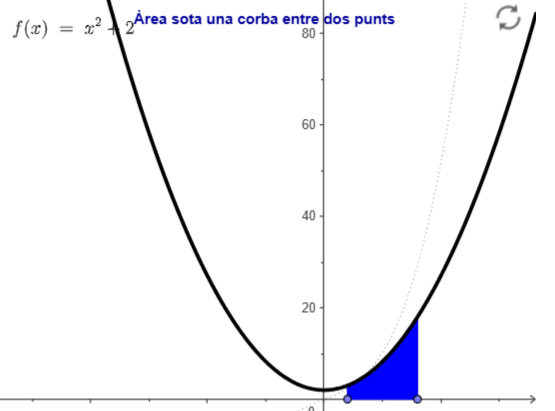
\includegraphics[width=0.6\textwidth]{area.png}
    \caption{Definició d'àrea sota la corba.}
    \label{fig:area}
\end{figure}

\subsection{Teorema fonamental del càlcul i Regla de Barrow}

El teorema fonamental del càlcul estableix la connexió entre derivades i integrals, i ens proporciona una manera pràctica de calcular integrals definides sense haver de recórrer a límits de sumes.

\begin{concept}
\textbf{Teorema fonamental del càlcul (1a part)}\\
Si $f$ és una funció contínua en un interval tancat $[a,b]$, la funció $F$ definida per:
\[
F(x) = \int_a^x f(t)\,dt
\]
és derivable en $(a,b)$ i:
\[
\boxed{\dfrac{dF}{dx} = f(x)}
\]
És a dir, la funció $F$ és una primitiva de $f$.
\end{concept}

\begin{concept}
\textbf{Teorema fonamental del càlcul (2a part) - Regla de Barrow}\\
Si $f$ és contínua en $[a,b]$ i $F$ és qualsevol primitiva de $f$ en aquest interval, aleshores:
\[
\boxed{\int_a^b f(x)\,dx = F(b) - F(a)}
\]
\end{concept}

\begin{exemple}
\textbf{Exemple: Càlcul d'una integral definida}\\
Calculem $\displaystyle \int_0^2 x^2\,dx$.

Una primitiva de $f(x)=x^2$ és $F(x)=\dfrac{x^3}{3}$. Aplicant la Regla de Barrow:
\[
\int_0^2 x^2\,dx = \left[\frac{x^3}{3}\right]_0^2 = \frac{2^3}{3} - \frac{0^3}{3} = \frac{8}{3}
\]
\end{exemple}

\subsection{Propietats de la integral definida}

\begin{concept}
\textbf{Propietats de la integral definida}
\begin{enumerate}
    \item \textbf{Linealitat:} $\displaystyle \int_a^b k\cdot f(x)\,dx = k\cdot \int_a^b f(x)\,dx$ (on $k$ és una constant).
    \item \textbf{Suma:} $\displaystyle \int_a^b (f(x) \pm g(x))\,dx = \int_a^b f(x)\,dx \pm \int_a^b g(x)\,dx$.
    \item \textbf{Additivitat respecte a l'interval:} Si $c \in [a,b]$, llavors:
    \[
    \int_a^b f(x)\,dx = \int_a^c f(x)\,dx + \int_c^b f(x)\,dx
    \]
    \item \textbf{Inversió de límits:} $\displaystyle \int_a^b f(x)\,dx = -\int_b^a f(x)\,dx$.
    \item \textbf{Integral de zero:} $\displaystyle \int_a^a f(x)\,dx = 0$.
\end{enumerate}
\end{concept}

\subsection{Àrea de recintes limitats per una funció entre dos punts i l'eix de les abscisses}

Un dels usos més importants de la integral definida és el càlcul d'àrees. Però cal tenir en compte que la integral definida dóna l'àrea \textbf{amb signe}. Per obtenir l'àrea (que sempre és positiva), hem de considerar el signe de la funció.

\begin{figure}[h]
    \centering
    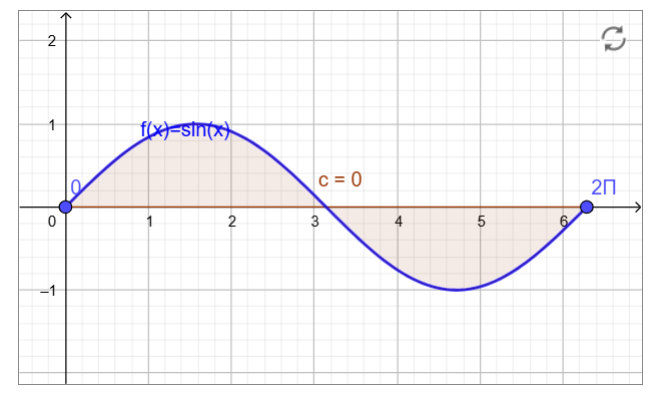
\includegraphics[width=0.6\textwidth]{areadospunts.png}
    \caption{Àrea de recintes limitats per una funció entre dos punts i l'eix de les abscisses.}
    \label{fig:area_dos_punts}
\end{figure}

\begin{concept}
\textbf{Precaució important:}\\
Quan la funció pren valors negatius en un interval, la integral definida en aquest interval és negativa. Per tant, per calcular l'àrea (que sempre és positiva), cal tenir en compte el signe de la funció:
\begin{itemize}
    \item Si $f(x) \ge 0$ en tot l'interval $[a,b]$, l'àrea és $\displaystyle \int_a^b f(x)\,dx$.
    \item Si $f(x) \le 0$ en tot l'interval $[a,b]$, l'àrea és $\displaystyle -\int_a^b f(x)\,dx = \left|\int_a^b f(x)\,dx\right|$.
    \item Si la funció canvia de signe dins de l'interval, cal dividir l'interval en subintervals on el signe sigui constant i sumar els valors absoluts de les integrals en cada subinterval.
\end{itemize}
\end{concept}

\begin{exemple}
\textbf{Exemple 1: Àrea entre $f(x)=\sin x$ i l'eix $OX$ entre $0$ i $2\pi$}\\
Per a calcular l'àrea, hem de dividir el gràfic en dues regions: $[0,\pi]$ i $[\pi,2\pi]$, ja que la funció s'anul·la a $x=\pi$.
\[
R_1 = \int_0^\pi \sin x\,dx = [-\cos x]_0^\pi = 2
\]
\[
R_2 = \left| \int_\pi^{2\pi} \sin x\,dx \right| = \left| [-\cos x]_\pi^{2\pi} \right| = 2
\]
Per tant, l'àrea total és:
\[
\boxed{A_{\text{total}} = R_1 + R_2 = 4}
\]
\end{exemple}

\begin{figure}[h]
    \centering
    % \includegraphics[width=0.6\textwidth]{area_sin.png}
    \caption{Àrea sota la corba de $f(x)=\sin x$ entre $0$ i $2\pi$. Cal calcular l'àrea per separat a cada costat de $\pi$ i sumar els valors absoluts.}
    \label{fig:area_sin}
\end{figure}

\begin{exemple}
\textbf{Exemple 2: Àrea entre $f(x)=x^2-4x+3$ i l'eix $OX$}\\
Calculem l'àrea de la regió limitada per la paràbola $f(x)=x^2-4x+3$ i l'eix $OX$.

Primer trobem els punts de tall amb l'eix $OX$:
\[
x^2-4x+3=0 \Rightarrow (x-1)(x-3)=0 \Rightarrow x=1, \quad x=3
\]
En l'interval $[1,3]$, la funció és negativa (la paràbola obre cap amunt i les arrels són 1 i 3). Per tant, l'àrea és:
\[
A = \left| \int_1^3 (x^2-4x+3)\,dx \right| = \left| \left[\frac{x^3}{3} - 2x^2 + 3x\right]_1^3 \right| = \left| 0 - \frac{4}{3} \right| = \frac{4}{3}
\]
\end{exemple}

\subsection{Àrea de recintes limitats per més d'una funció}

Quan l'àrea que volem calcular està limitada per dues o més funcions, el procés és similar però amb una diferència clau: en lloc de calcular l'àrea sota una funció i l'eix, calculem l'àrea entre les dues funcions.

\begin{figure}[h]
    \centering
    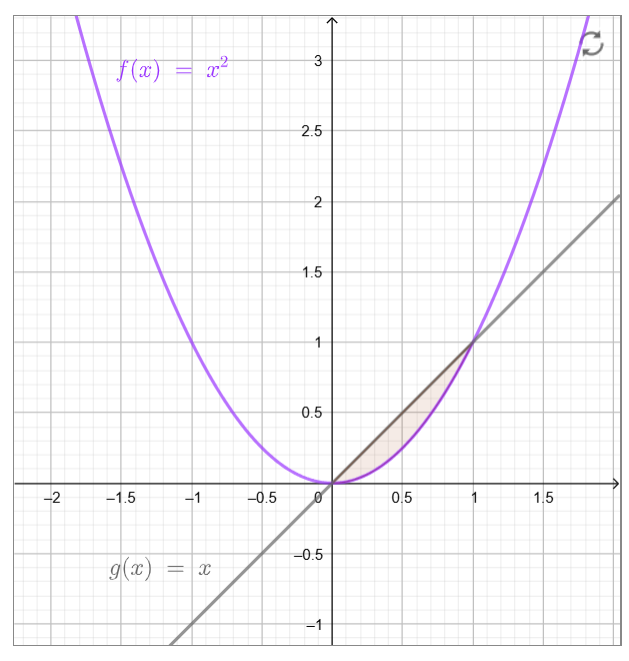
\includegraphics[width=0.6\textwidth]{areaduesfuncions.png}
    \caption{Àrea de recintes limitats per més d'una funció}
    \label{fig:areadues}
\end{figure}

\begin{concept}
\textbf{Àrea entre dues corbes}\\
Donades dues funcions contínues $f(x)$ i $g(x)$ en un interval $[a,b]$, l'àrea de la regió compresa entre les dues corbes és:
\[
\boxed{A = \int_a^b \left( f_{\text{superior}}(x) - f_{\text{inferior}}(x) \right) dx}
\]
on $f_{\text{superior}}$ és la funció que es troba per sobre de l'altra en l'interval considerat.
\end{concept}

\textbf{Passos per calcular l'àrea entre dues corbes:}
\begin{enumerate}
    \item \textbf{Trobar els punts de tall} de les funcions (igualar-les i resoldre per $x$).
    \item \textbf{Determinar quina funció és més gran} en cada interval (avaluant un punt qualsevol).
    \item \textbf{Calcular la integral} de la diferència entre la funció superior i la inferior, entre els punts de tall.
\end{enumerate}

\begin{figure}[h]
    \centering
    % \includegraphics[width=0.6\textwidth]{area_entre_corbes.png}
    \caption{Àrea compresa entre dues corbes. L'àrea buscada és la diferència entre l'àrea sota la funció superior i l'àrea sota la funció inferior.}
    \label{fig:area_entre_corbes}
\end{figure}

\begin{exemple}
\textbf{Exemple 3: Àrea compresa entre $f(x)=x^2$ i $g(x)=x$}\\
Primer trobem els punts de tall:
\[
x^2 = x \Rightarrow x(x-1)=0 \Rightarrow x=0, \quad x=1
\]
En l'interval $[0,1]$, la funció $g(x)=x$ és més gran que $f(x)=x^2$ (per exemple, a $x=0.5$, $0.5 > 0.25$).

L'àrea és:
\[
A = \int_0^1 (x - x^2)\,dx = \left[\frac{x^2}{2} - \frac{x^3}{3}\right]_0^1 = \frac{1}{2} - \frac{1}{3} = \frac{1}{6}
\]
\end{exemple}

\begin{exemple}
\textbf{Exemple 4: Àrea compresa entre $f(x)=x^2$ i $g(x)=2x-x^2$}\\
Trobem els punts de tall:
\[
x^2 = 2x - x^2 \Rightarrow 2x^2 - 2x = 0 \Rightarrow 2x(x-1)=0 \Rightarrow x=0, \quad x=1
\]
En l'interval $[0,1]$, $g(x)=2x-x^2$ és més gran que $f(x)=x^2$ (per exemple, a $x=0.5$, $0.75 > 0.25$).

L'àrea és:
\[
A = \int_0^1 \left( (2x-x^2) - x^2 \right) dx = \int_0^1 (2x - 2x^2)\,dx = \left[x^2 - \frac{2x^3}{3}\right]_0^1 = 1 - \frac{2}{3} = \frac{1}{3}
\]
\end{exemple}

\begin{exemple}
\textbf{Exemple 5: Àrea compresa entre $y=x^2$ i la recta $y=x+2$}\\
Trobem els punts de tall:
\[
x^2 = x+2 \Rightarrow x^2 - x - 2 = 0 \Rightarrow (x-2)(x+1)=0 \Rightarrow x=-1, \quad x=2
\]
En l'interval $[-1,2]$, la recta $y=x+2$ és més gran que la paràbola $y=x^2$ (per exemple, a $x=0$, $2>0$).

L'àrea és:
\[
A = \int_{-1}^2 \left( (x+2) - x^2 \right) dx = \left[\frac{x^2}{2} + 2x - \frac{x^3}{3}\right]_{-1}^2 = \frac{9}{2}
\]
\end{exemple}

% ---------------------------------------------------------
% NOVA SECCIÓ: APLICACIONS DE LA INTEGRAL DEFINIDA
% ---------------------------------------------------------
\subsection{Aplicacions de la integral definida}

La integral definida no només serveix per calcular àrees. A continuació mostrem dues aplicacions habituals: el càlcul de volums de sòlids de revolució i el càlcul del treball realitzat per una força variable.

\subsubsection*{Volum d'un sòlid de revolució}

Quan fem girar una regió plana al voltant d'un eix, obtenim un sòlid de revolució. El volum d'aquest sòlid es pot calcular mitjançant la fórmula dels discs (o de les arestes). Per a una funció $f(x) \ge 0$ en $[a,b]$, el volum generat en girar la regió sota la corba al voltant de l'eix $OX$ és:
\[
\boxed{V = \pi \int_a^b [f(x)]^2\,dx}
\]

\begin{exemple}
\textbf{Exemple: Volum d'una esfera}\\
Calculem el volum de l'esfera de radi $R$ generada per la semicircumferència $f(x) = \sqrt{R^2 - x^2}$ (per $x \in [-R,R]$) en girar al voltant de l'eix $OX$:
\[
V = \pi \int_{-R}^{R} (R^2 - x^2)\,dx = \pi \left[ R^2 x - \frac{x^3}{3} \right]_{-R}^{R} = \pi \left( R^3 - \frac{R^3}{3} - \left(-R^3 + \frac{R^3}{3}\right) \right) = \frac{4}{3}\pi R^3
\]
\end{exemple}

\subsubsection*{Treball realitzat per una força variable}

En física, el treball realitzat per una força variable $F(x)$ que actua al llarg d'un desplaçament de $a$ a $b$ és:
\[
\boxed{W = \int_a^b F(x)\,dx}
\]

\begin{exemple}
\textbf{Exemple: Treball per estirar una molla}\\
Segons la llei de Hooke, la força necessària per estirar una molla una distància $x$ des de la posició d'equilibri és $F(x) = kx$, on $k$ és la constant de la molla. Per estirar la molla des de $x=0$ fins a $x=L$, el treball realitzat és:
\[
W = \int_0^L kx\,dx = \frac{1}{2}kL^2
\]
\end{exemple}


% ---------------------------------------------------------
% EXERCICIS FINALS
% ---------------------------------------------------------
\section{Exercicis finals}

\subsection{Exercicis d'integrals indefinides}

\begin{exercici}
Calcula les següents integrals indefinides:
\begin{enumerate}
    \item $\displaystyle \int (3x^2 - 2x + 5)\,dx$
    \item $\displaystyle \int \dfrac{1}{x}\,dx$
    \item $\displaystyle \int e^x\,dx$
    \item $\displaystyle \int \sin x\,dx$
    \item $\displaystyle \int \cos x\,dx$
\end{enumerate}
\end{exercici}

\begin{exercici}
Calcula les següents integrals quasi-immediates:
\begin{enumerate}
    \item $\displaystyle \int \dfrac{x}{x^2+1}\,dx$
    \item $\displaystyle \int x e^{x^2}\,dx$
    \item $\displaystyle \int \sin x \cos x\,dx$
    \item $\displaystyle \int \dfrac{\cos x}{\sin x}\,dx$
    \item $\displaystyle \int \dfrac{1}{\sqrt{1-x^2}}\,dx$
\end{enumerate}
\end{exercici}

\subsection{Exercicis de mètodes d'integració}

\begin{exercici}
Calcula les següents integrals racionals:
\begin{enumerate}
    \item $\displaystyle \int \dfrac{1}{x^2-1}\,dx$
    \item $\displaystyle \int \dfrac{1}{x^2+4x+5}\,dx$
    \item $\displaystyle \int \dfrac{x+1}{x^2+2x+5}\,dx$
    \item $\displaystyle \int \dfrac{x^2}{x+1}\,dx$
    \item $\displaystyle \int \dfrac{2x+3}{x^2-3x+2}\,dx$
\end{enumerate}
\end{exercici}

\begin{exercici}
Calcula les següents integrals per parts:
\begin{enumerate}
    \item $\displaystyle \int x e^x\,dx$
    \item $\displaystyle \int x \sin x\,dx$
    \item $\displaystyle \int \ln x\,dx$
    \item $\displaystyle \int x^2 e^x\,dx$
    \item $\displaystyle \int x \cos(2x)\,dx$
\end{enumerate}
\end{exercici}

\begin{exercici}
Calcula les següents integrals utilitzant un canvi de variable:
\begin{enumerate}
    \item $\displaystyle \int \dfrac{dx}{x\sqrt{x^2-1}}$
    \item $\displaystyle \int \sqrt{9-x^2}\,dx$
    \item $\displaystyle \int \dfrac{e^x}{e^x+1}\,dx$
    \item $\displaystyle \int \dfrac{1}{1+\sin x}\,dx$
    \item $\displaystyle \int \dfrac{1}{1+\cos x}\,dx$
\end{enumerate}
\end{exercici}

\subsection{Exercicis d'integrals definides i àrees}

\begin{exercici}
Calcula les següents integrals definides:
\begin{enumerate}
    \item $\displaystyle \int_0^1 x^2\,dx$
    \item $\displaystyle \int_0^\pi \sin x\,dx$
    \item $\displaystyle \int_1^e \dfrac{1}{x}\,dx$
    \item $\displaystyle \int_0^1 e^x\,dx$
\end{enumerate}
\end{exercici}

\begin{exercici}
Calcula l'àrea del recinte limitat per:
\begin{enumerate}
    \item La funció $f(x)=x^2-4x+3$ i l'eix $OX$ entre $x=1$ i $x=3$.
    \item La funció $f(x)=\cos x$ i l'eix $OX$ entre $x=0$ i $x=2\pi$.
    \item Les funcions $f(x)=x^2$ i $g(x)=2x-x^2$.
    \item La paràbola $y=x^2$ i la recta $y=x+2$.
\end{enumerate}
\end{exercici}

% ---------------------------------------------------------
% NOVA SECCIÓ: SOLUCIONARI
% ---------------------------------------------------------
\section*{Solucionari dels exercicis finals}
\addcontentsline{toc}{section}{Solucionari}

\subsection*{Exercicis d'integrals indefinides (secció 5.1)}

\begin{solucio}
\begin{enumerate}
    \item $\displaystyle \int (3x^2 - 2x + 5)\,dx = x^3 - x^2 + 5x + C$
    \item $\displaystyle \int \dfrac{1}{x}\,dx = \ln|x| + C$
    \item $\displaystyle \int e^x\,dx = e^x + C$
    \item $\displaystyle \int \sin x\,dx = -\cos x + C$
    \item $\displaystyle \int \cos x\,dx = \sin x + C$
\end{enumerate}
\end{solucio}

\begin{solucio}
\begin{enumerate}
    \item $\displaystyle \int \dfrac{x}{x^2+1}\,dx = \frac{1}{2}\ln(x^2+1) + C$
    \item $\displaystyle \int x e^{x^2}\,dx = \frac{1}{2}e^{x^2} + C$
    \item $\displaystyle \int \sin x \cos x\,dx = \frac{1}{2}\sin^2 x + C$ (o $-\frac{1}{2}\cos^2 x + C$)
    \item $\displaystyle \int \dfrac{\cos x}{\sin x}\,dx = \ln|\sin x| + C$
    \item $\displaystyle \int \dfrac{1}{\sqrt{1-x^2}}\,dx = \arcsin x + C$
\end{enumerate}
\end{solucio}

\subsection*{Exercicis de mètodes d'integració (secció 5.2)}

\begin{solucio}
\begin{enumerate}
    \item $\displaystyle \int \dfrac{1}{x^2-1}\,dx = \frac{1}{2}\ln\left|\frac{x-1}{x+1}\right| + C$ (fraccions parcials)
    \item $\displaystyle \int \dfrac{1}{x^2+4x+5}\,dx = \arctan(x+2) + C$ (completant quadrats: $(x+2)^2+1$)
    \item $\displaystyle \int \dfrac{x+1}{x^2+2x+5}\,dx = \frac{1}{2}\ln(x^2+2x+5) + C$ (derivada del denominador és $2x+2$)
    \item $\displaystyle \int \dfrac{x^2}{x+1}\,dx = \frac{x^2}{2} - x + \ln|x+1| + C$ (divisió prèvia)
    \item $\displaystyle \int \dfrac{2x+3}{x^2-3x+2}\,dx = 7\ln|x-2| - 5\ln|x-1| + C$ (fraccions parcials: $A=7$, $B=-5$)
\end{enumerate}
\end{solucio}

\begin{solucio}
\begin{enumerate}
    \item $\displaystyle \int x e^x\,dx = e^x(x-1) + C$
    \item $\displaystyle \int x \sin x\,dx = -x\cos x + \sin x + C$
    \item $\displaystyle \int \ln x\,dx = x\ln x - x + C$
    \item $\displaystyle \int x^2 e^x\,dx = e^x(x^2 - 2x + 2) + C$
    \item $\displaystyle \int x \cos(2x)\,dx = \frac{x}{2}\sin(2x) + \frac{1}{4}\cos(2x) + C$
\end{enumerate}
\end{solucio}

\begin{solucio}
\begin{enumerate}
    \item $\displaystyle \int \dfrac{dx}{x\sqrt{x^2-1}} = \arctan(\sqrt{x^2-1}) + C$
    \item $\displaystyle \int \sqrt{9-x^2}\,dx = \frac{9}{2}\arcsin\left(\frac{x}{3}\right) + \frac{x}{2}\sqrt{9-x^2} + C$
    \item $\displaystyle \int \dfrac{e^x}{e^x+1}\,dx = \ln(e^x+1) + C$
    \item $\displaystyle \int \dfrac{1}{1+\sin x}\,dx = \tan x - \sec x + C$ (p. ex., multiplicant per $1-\sin x$)
    \item $\displaystyle \int \dfrac{1}{1+\cos x}\,dx = \tan\left(\frac{x}{2}\right) + C$ (o $-\cot(x/2)$ depenent de la convenció)
\end{enumerate}
\end{solucio}

\subsection*{Exercicis d'integrals definides i àrees (secció 5.3)}

\begin{solucio}
\begin{enumerate}
    \item $\displaystyle \int_0^1 x^2\,dx = \frac{1}{3}$
    \item $\displaystyle \int_0^\pi \sin x\,dx = 2$
    \item $\displaystyle \int_1^e \dfrac{1}{x}\,dx = 1$
    \item $\displaystyle \int_0^1 e^x\,dx = e - 1$
\end{enumerate}
\end{solucio}

\begin{solucio}
\begin{enumerate}
    \item Àrea entre $f(x)=x^2-4x+3$ i l'eix $OX$ entre $1$ i $3$: $\dfrac{4}{3}$.
    \item Àrea entre $\cos x$ i l'eix $OX$ entre $0$ i $2\pi$: $4$ (divideix en $[0,\pi/2]$, $[\pi/2,3\pi/2]$, $[3\pi/2,2\pi]$ i suma els valors absoluts).
    \item Àrea entre $f(x)=x^2$ i $g(x)=2x-x^2$: $\dfrac{1}{3}$.
    \item Àrea entre $y=x^2$ i $y=x+2$: $\dfrac{9}{2}$.
\end{enumerate}
\end{solucio}

\end{document}